%% V1.0
%% by Gabriel Garcia, gabrcg@gmail.com
%% This is a template for Udacity projects using IEEEtran.cls

%% Be Udacious!

\documentclass[10pt,journal,compsoc]{IEEEtran}

\usepackage[pdftex]{graphicx}    
\usepackage{cite}
\hyphenation{op-tical net-works semi-conduc-tor}


\begin{document}

\title{Robotic Inference}

\author{Seyfi Gozubuyuk}

\markboth{Inference project, Robotic Nanodegree, Udacity}%
{}
\IEEEtitleabstractindextext{%

\begin{abstract}
Deep Learning is widely used in object classification. Convolutional Neural Networks improved the success of the computers on object detection, recognition, and classification. They are commonly used in Self-Driving Cars, robotics and other fields of machine learning. There exist models such as LeNet, AlexNet, and GoogleNet. Nvidia Digits provides a web interface to utilize these models and create other models.  It is possible to upload data and test it with these models. This project includes different classification tasks on image datasets. 
\end{abstract}

% Note that keywords are not normally used for peerreview papers.
\begin{IEEEkeywords}
Robot, IEEEtran, Udacity, \LaTeX, Deep Learning, Convolutional Neural Networks, Nvidia Digits.
\end{IEEEkeywords}}


\maketitle
\IEEEdisplaynontitleabstractindextext
\IEEEpeerreviewmaketitle
\section{Introduction}
\label{sec:introduction}

\IEEEPARstart{T}{he} goal in this project is to utilize Nvidia Digits application to perform classification on image datasets. There are two datasets. The first one is the provided data that contains bottle and candy box images. Besides, there exist samples that do not include any.\\
The second dataset was The German Traffic Sign dataset\cite{tsign}. There are 43 different traffic signs. This dataset was selected because it is related with self-driving field and it has many different classes.\\
Nvidia Digits provide an interface to load the data, create a new model or utilize predefined models. Besides, it enables to customize the models and select hyperparameters. During training, it saves the model on every epoch. This saved models can be used as pretrained models to train more.

\section{Background / Formulation}
The problem is to classify objects using Deep Learning. Convolutional neural networks are an excellent choice \cite{wiki:cnn}. Backpropagation provided enhanced learning for Multilayer Neural Networks.\\
LeCun et al. developed LeNet to classify digits in 1998\cite{lenet}. LeNet was a seven-layer CNN. Krizhevsky et al. built a convolutional neural network which has sixty million parameters, half million neurons and five convolutional layers in 2012 \cite{AlexNet}. Szegedy et al. trained another deep neural network in 2014 which has 22 layers \cite{gnet}.

\subsection{Task 1: Bottle vs Candy-Box}
In the first task, AlexNet and GoogleNet were selected to classify the samples of bottles and candy-boxes. The reason for choosing AlexNet is its speed, and the reason for working with the GoogleNet was its higher accuracy. Five different models trained while completing this task. Since adam and RMSprop help the gradient descent to reach the minima faster, these solver types were allied with AlexNet and GoogleNet. Besides the Stochastic Gradient Descent were selected with AlexNet as the default option. Learning rate 0.01 was a reasonable choice to prevent overfitting and from overshooting. The image sizes were compatible with AlexNet and GoogleNet. Therefore there were no changes in dimensions. The number of epochs parameter has different values to experiment. The results section discuss the details of the models tried and the outcomes.

\subsection{Task 2: Traffic Sign}
The selected dataset has 39,209 images in 43 classes for training. Besides, there are 12,530 images to test. The image size is varying between 15x15 and 250x250 pixels. This situation forced the use of LeNet. All samples were resized by squashing to 28x28 during loading. Enlarging the images would result in excessive training. From the experience from the first task, the solver type was selected as stochastic gradient descent. The learning rate was again 0.01 since it provided satisfying results in the previous part of the project.

\section{Data Acquisition}
The first task does not contain any changes on the data, since the models were compatible with image size of 256x256.


The second task works on the traffic signs data. The main reasons are to select a dataset related to autonomous vehicles and to select a dataset with many classes. A problem with the dataset was, it had varying image sizes, and these sizes were small to use AlexNet or GoogleNet. Therefore, the LeNet model was the remaining choice for this part of the project. Since LeNet takes input grayscales images with size 28x28, all images in the dataset were resized to 28x28 and converted to grayscale. Nvidia Digits automatically performed these operations during loading the data. The number of epochs was selected as ten to prevent overfitting.\\
Figure~\ref{fig:tss14} shows samples from 14 different classes.
\begin{figure}[thpb]
      \centering
      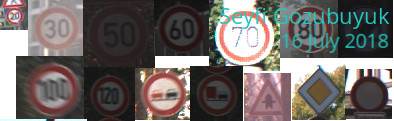
\includegraphics[width=\linewidth]{figures/Tsignsamples14.png}
      \caption{Samples From 14 Different Classes}
      \label{fig:tss14}
\end{figure}

\section{Results}
\subsection{Task 1: Bottle vs Candy-Box}
The results for the five different model for the Task 1 are given on Table~\ref{table:t1r}.

\begin{table}[h]
\caption{Results on Task 1}
\label{table:t1r}
\begin{center}
\begin{tabular}{|c||c||c||c||c||c||c|}
\hline
No. & Model & Epoc & Solver & Rate & Accuracy \\
\hline
1* & AlexNet1 & 30 & RSMprop & 0.01 & 73.77\%\\
\hline
2* & AlexNet1E17 & 5 & RSMprop & 0.0001 & 70.49\%\\
\hline
3 & GoogleNet & 6 & Adam & 0.01 & 67.21\%\\
\hline
4* & GoogleNetE6 & 4 & Adam & 0.01 & 67.21\%\\
\hline
5 & AlexNet2 & 10 & SGD & 0.01 & 75.41\%\\
\hline
\end{tabular}
\end{center}
1* RMS decay value for 1.AlexNet1 and 2.AlexNet1E17 were 0.99\\
2* AlexNet1E17 started from the Epoch 17 of model 1.AlexNet1\\
4* GoogleNetE6 started from the Epoch 6 of model 3.GoogleNet
\end{table}

Figure~\ref{fig:t1a2c} shows the screenshot of the console when evaluating the AlexNet2 model for Task1.

\begin{figure}[thpb]
      \centering
      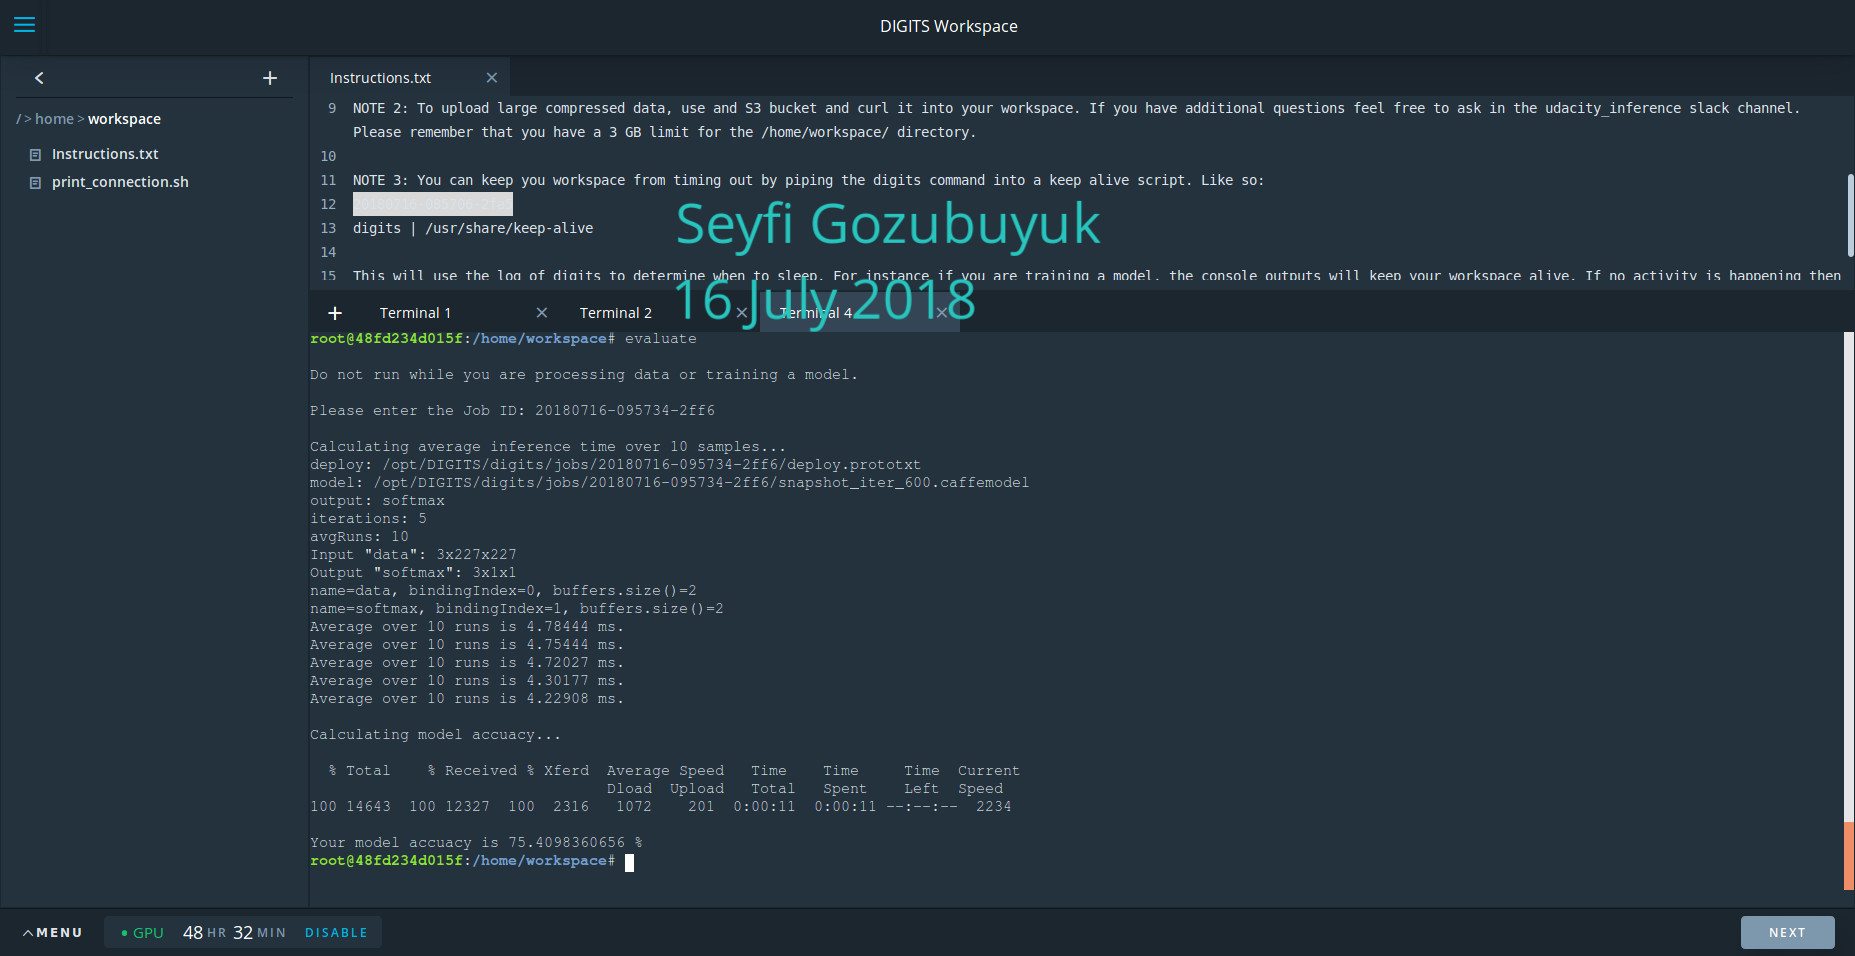
\includegraphics[width=\linewidth]{figures/t1a2c.png}
      \caption{Screenshot of Task 1 AlexNet2}
      \label{fig:t1a2c}
\end{figure}

Figure~\ref{fig:t1a2g} shows the training graph of successful AlexNet2 model. Figure~\ref{fig:t1a2l}, Figure~\ref{fig:t1a2t1}, Figure~\ref{fig:t1a2t2}, and Figure~\ref{fig:t1a2t3} shows the classification results of testing AlexNet2.

\begin{figure}[thpb]
      \centering
      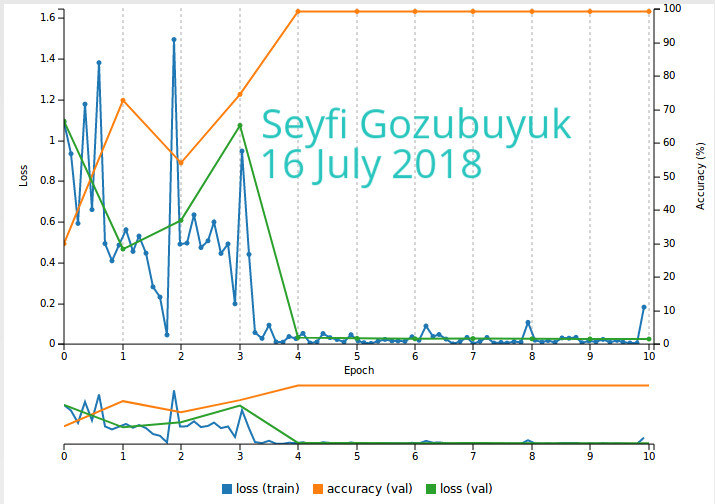
\includegraphics[width=\linewidth]{figures/t1a2g.png}
      \caption{Training Graph of Task 1 AlexNet2}
      \label{fig:t1a2g}
\end{figure}

\begin{figure}[thpb]
      \centering
      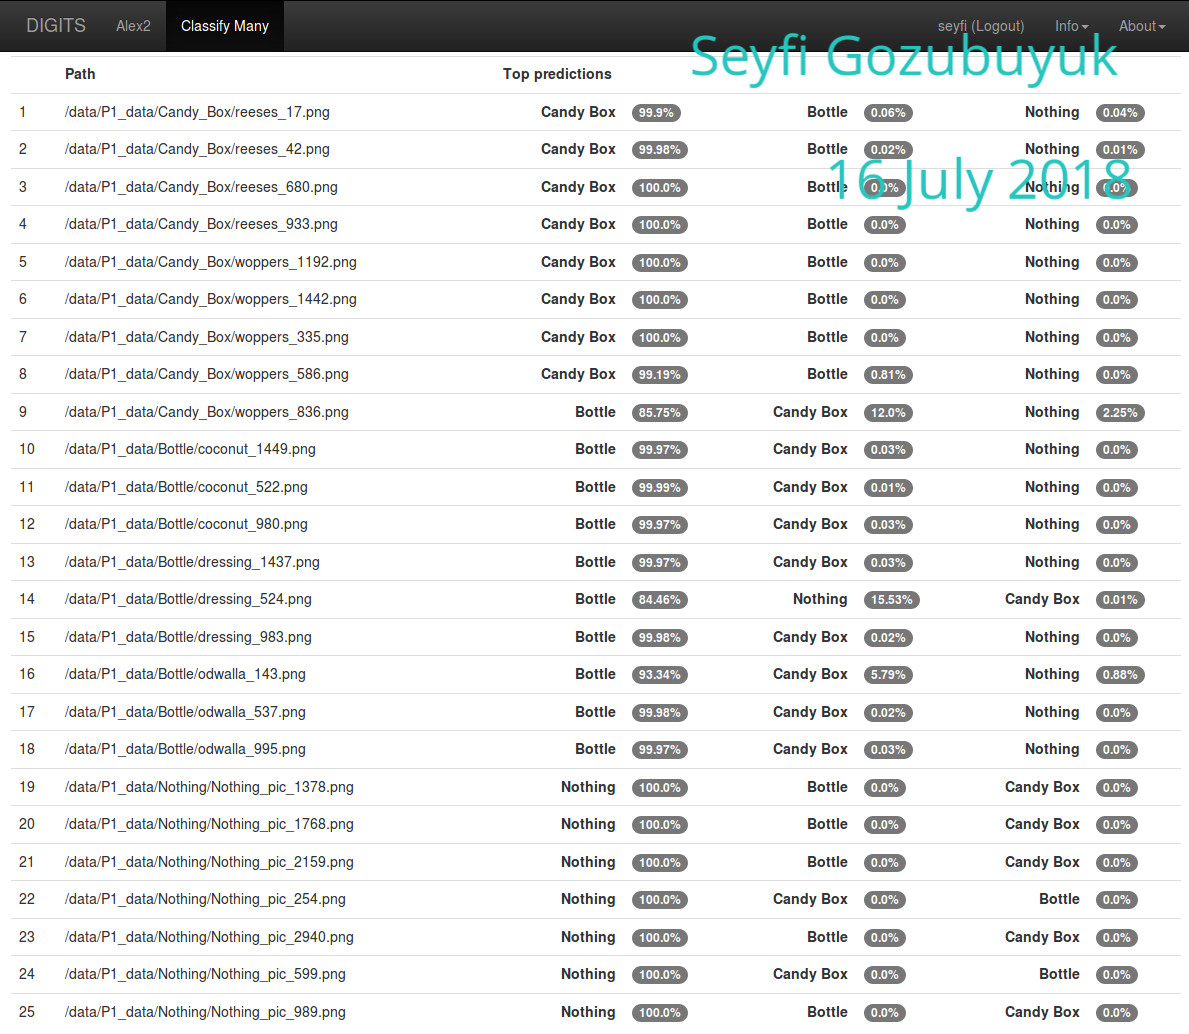
\includegraphics[width=\linewidth]{figures/t1a2l.png}
      \caption{Testing 25 Images with Task 1 AlexNet2}
      \label{fig:t1a2l}
\end{figure}


\begin{figure}[thpb]
      \centering
      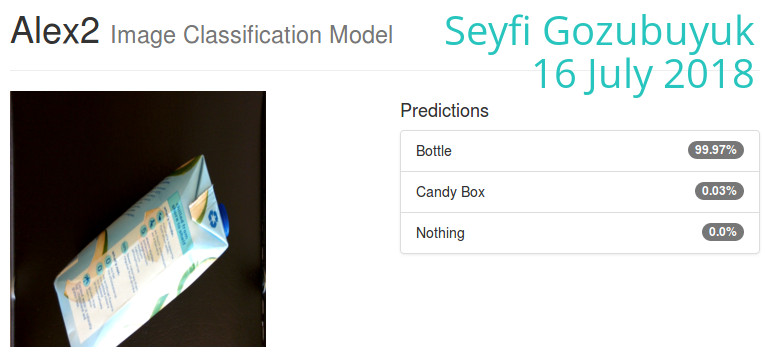
\includegraphics[width=\linewidth]{figures/t1a2t1.png}
      \caption{Testing a Bottle Image Task 1 AlexNet2}
      \label{fig:t1a2t1}
\end{figure}


\begin{figure}[thpb]
      \centering
      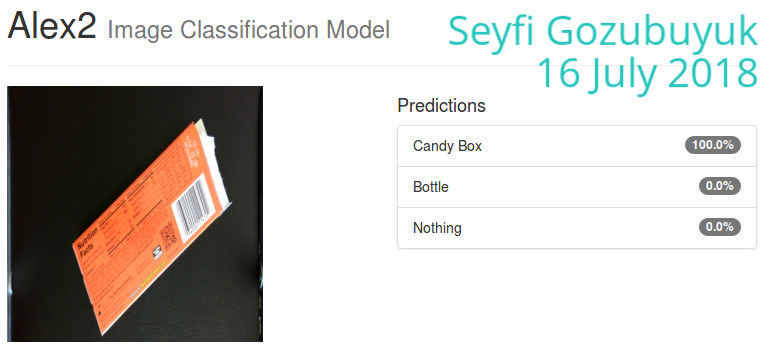
\includegraphics[width=\linewidth]{figures/t1a2t2.png}
      \caption{Testing a Candy-Box Image Task 1 AlexNet2}
      \label{fig:t1a2t2}
\end{figure}


\begin{figure}[thpb]
      \centering
      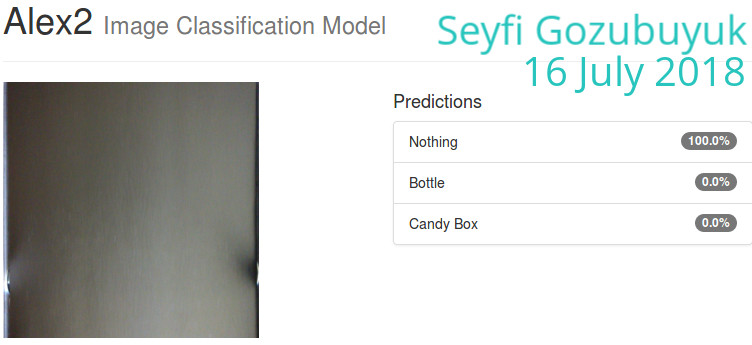
\includegraphics[width=\linewidth]{figures/t1a2t3.png}
      \caption{Testing a Nothing Image Task 1 AlexNet2}
      \label{fig:t1a2t3}
\end{figure}



Figure~\ref{fig:t1a1g} shows the training graph of unsuccessful AlexNet1 model. The accuracy graph shows that the highest accuracy was obtained at epoch 17.

\begin{figure}[thpb]
      \centering
      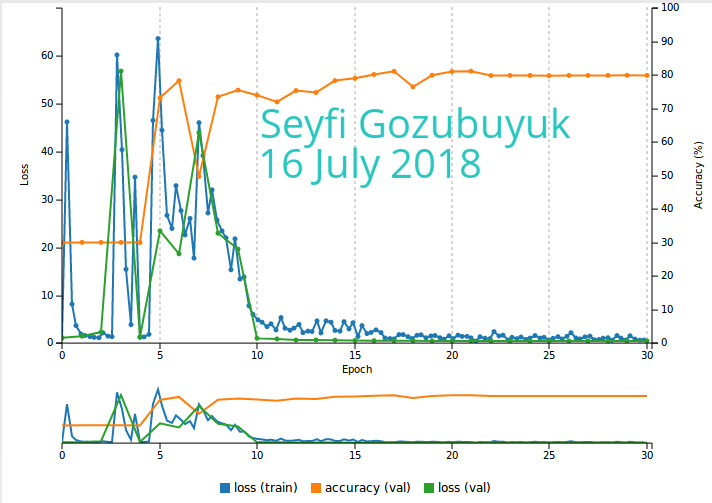
\includegraphics[width=\linewidth]{figures/t1a1g.png}
      \caption{Training Graph of Task 1 AlexNet1}
      \label{fig:t1a1g}
\end{figure}

\subsection{Task 2: Traffic Sign}
Figure ~\ref{fig:t2g} show the training graph of the LeNet for the second task. It can be seen from the graph that, the accuracy did not change significantly after ten epochs. The validation accuracy at tenth epoch was 98.7276\% and for the thirtieth epoch 98.7581\%. The highest accuracy was 98.7785\% for the nineteenth epoch. 

\begin{figure}[thpb]
      \centering
      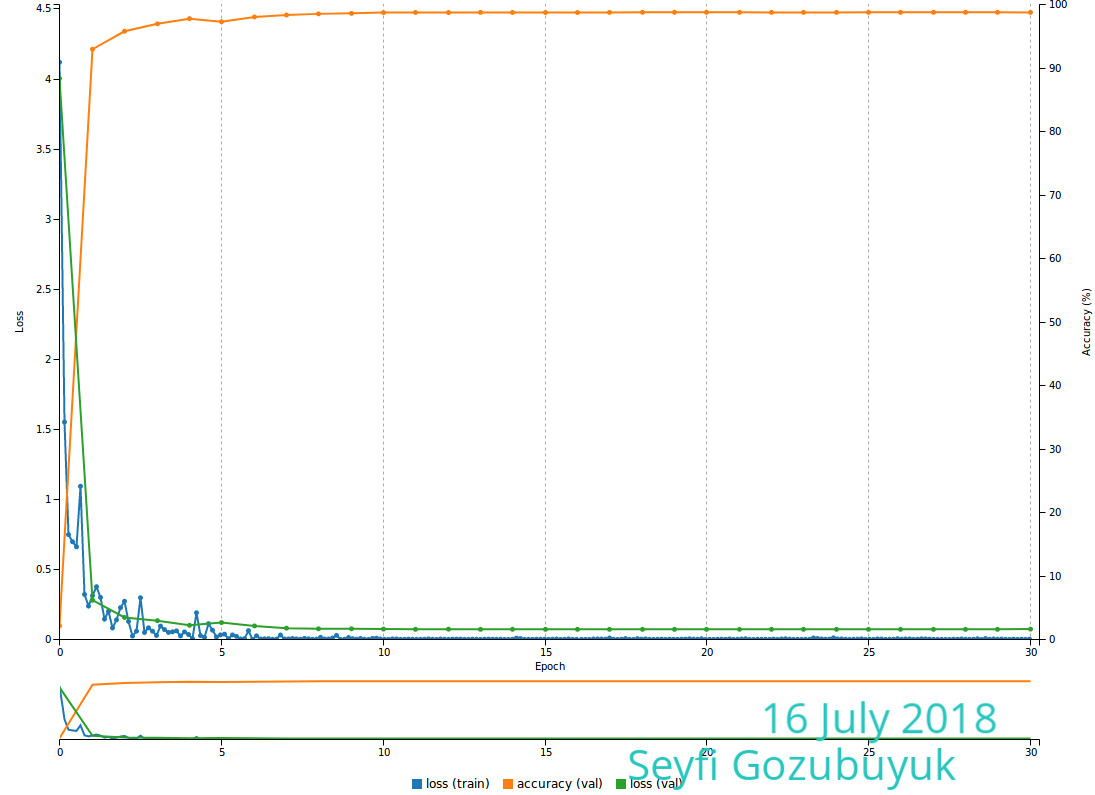
\includegraphics[width=\linewidth]{figures/t2g.png}
      \caption{Training Graph of Task 2 LeNet}
      \label{fig:t2g}
\end{figure}

Figure ~\ref{fig:t2tnpc} shows the top 9 predictions for category. Figure ~\ref{fig:t2t1}, Figure ~\ref{fig:t2t2}, and Figure ~\ref{fig:t2t3} shows sample difficult predictions.

\begin{figure}[thpb]
      \centering
      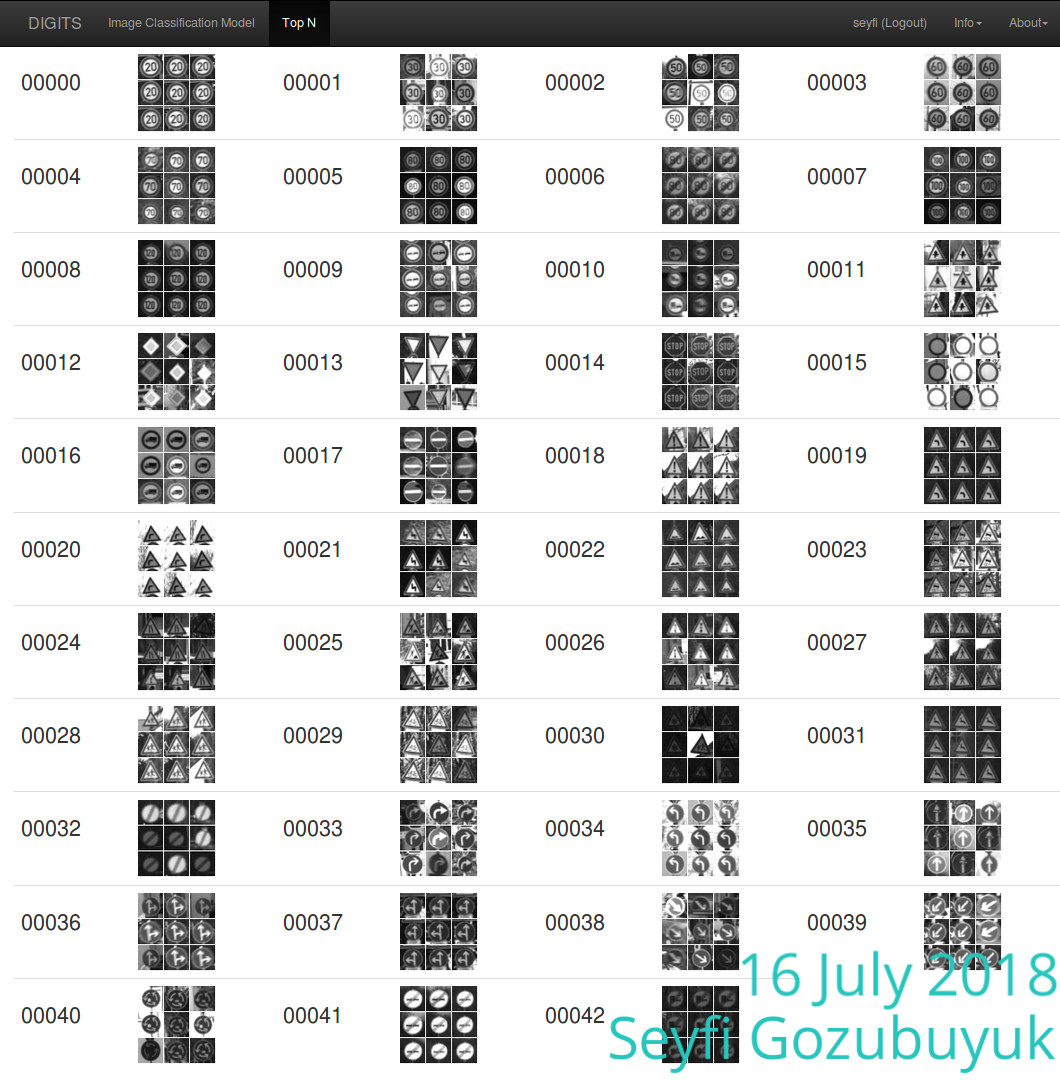
\includegraphics[width=\linewidth]{figures/TopNperCat.png}
      \caption{Top 9 Predictions per Category}
      \label{fig:t2tnpc}
\end{figure}


\begin{figure}[thpb]
      \centering
      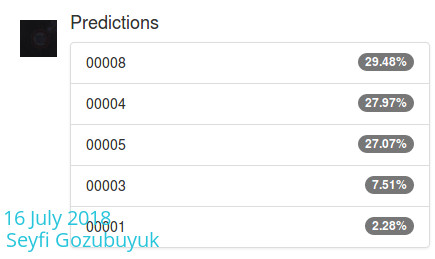
\includegraphics[width=\linewidth]{figures/t2t1.png}
      \caption{Traffic Sign Test 1}
      \label{fig:t2t1}
\end{figure}


\begin{figure}[thpb]
      \centering
      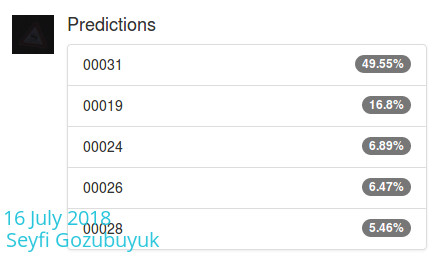
\includegraphics[width=\linewidth]{figures/t2t2.png}
      \caption{Traffic Sign Test 2}
      \label{fig:t2t2}
\end{figure}

\begin{figure}[thpb]
      \centering
      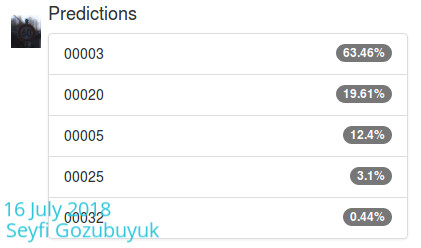
\includegraphics[width=\linewidth]{figures/t2t3.png}
      \caption{Traffic Sign Test 3}
      \label{fig:t2t3}
\end{figure}

\section{Discussion}
The Figure ~\ref{fig:t1a1g} and Figure ~\ref{fig:t1a2g} show that SGD worked better on both the validation dataset and the test dataset for the Task 1. The GoogleNet was not successful for this dataset. The reason was the use of Adam optimizer instead of SGD and the small number of epochs. It is required to either increase the number of epochs or select the SGD optimizer.\\

For the second task, due to time and hardware limitations, the available datasets were limited. Most of the datasets for autonomous driving have larger than 10 GB data sizes. The Traffic Sign Classification is an old problem, and there are already excellent results. In addition, the size of the images in the dataset made use of AlexNet or GoogleNet irrational. Besides, the LeNet already provide satisfactory results.

\section{Conclusion / Future work}
The results of the first task are open for improvement. A deeper network or optimized hyperparameters may provide better accuracy. Due to time limitations, this remains as future work.\\

For the second part of the project, it is required to access an environment which has more than 10 GB disk space and a GPU with more than 4 GB memory. As a future work, deeper networks will be trained for more complex datasets such as vehicle and pedestrian detection.\\

Testing the trained networks on a Jetson TX2 is another waiting task.

\subsection{Hardware Deployment}
The first part of the project was deployed on Udacity Workspace. Udacity Workspace provides a powerful GPU, which offers fast training and enough memory to train large deep networks.
The second part of the project was deployed in the local installation of Nvidia Digits. The machine has an I7 CPU, 8GB RAM, and 650M GPU. The configuration was able to train LeNet, and with more powerful CPU and GPU, it will be possible to increase the complexity of the network. 

\bibliography{bib}
\bibliographystyle{ieeetr}

\end{document}